\subsection{PIMS Space Module}
This module is responsible for providing all the core functionality of Patient Information Management System. The front-end component displays all the available services to the user. \par 

\subsubsection{Scope}
The scope is shown in the use case diagram below: \par
		\begin{figure}[H]
			\centerline{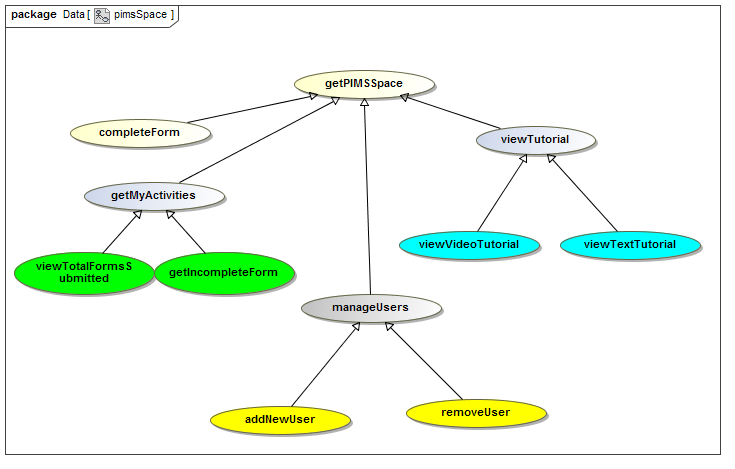
\includegraphics[width=0.75\linewidth]{./Functional_Requirements/Graphics/pimsSpace/pimsSpace}}
			\caption{Scope for PIMS Space Module}
		\end{figure}

\subsubsection{Use cases}
\begin{description}
	\item{\textbf{getPIMSSpace:}}
		\begin{description} Provides the user with the front-end of the PIMS; two spaces exist given the user's privileges. If a user is an administrator, they are provided with a space with features designed for them. The same applies for normal uses, who have fewer features than the administrator.
		\item{\textbf{Service Contract}} Below is a detailed service contract of how a PIMS Space is provided to the user and the actions that follow their requests.
		\begin{figure}[H]
			\centerline{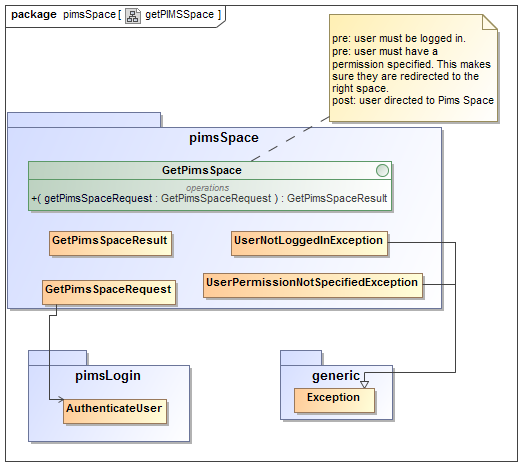
\includegraphics[width=0.7\linewidth]{./Functional_Requirements/Graphics/pimsSpace/getPIMSSpace}}
			\caption{Service contract for getPIMSSpace}
		\end{figure}
	\end{description} 
	\item{completeAndSubmitForm:} Allows the user to complete and submit forms to the database, provided all the required fields are complete and the data type match the required ones.
			\begin{description}
		\item{\textbf{Service Contract}} The service contract below further explains how completeAndSubmitForm works.
		\begin{figure}[H]
			\centerline{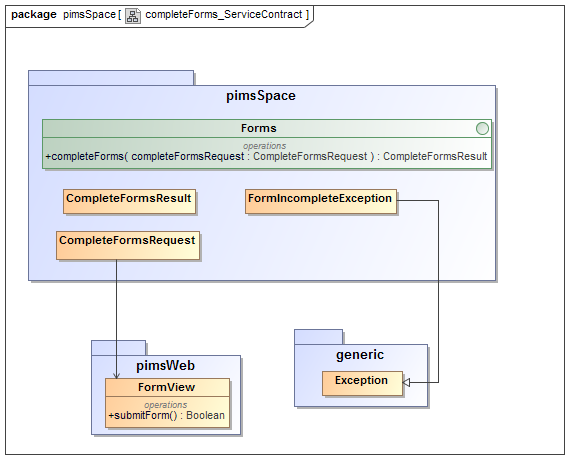
\includegraphics[width=0.7\linewidth]{./Functional_Requirements/Graphics/pimsSpace/completeForms_ServiceContract}}
			\caption{Service contract for completeForm}
		\end{figure}
	\end{description} 
	\item{viewTutorial:} This provides users with a different tutorials: a video tutorial that covers all the core functionality, an image tutorial with the most critical functionality, and a user-manual that provides a detailed explanation of PIMS.
	\item{addNewUser:} This functionality is only for the administrator; normal users cannot access this page and are redirected to their respective PIMS space. This allows for the addition of new users to the system; access rights are also
			\begin{description}
		\item{\textbf{Service Contract}} Below is the service contract, outlining the aforementioned.
		\begin{figure}[H]
			\centerline{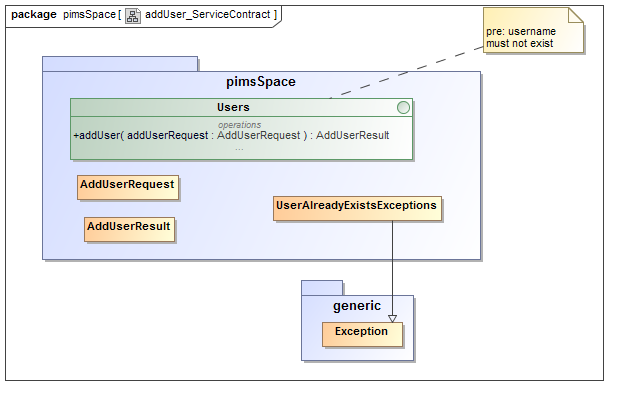
\includegraphics[width=0.7\linewidth]{./Functional_Requirements/Graphics/pimsSpace/addUser_ServiceContract}}
			\caption{Service contract for addNewUser}
		\end{figure}
	\end{description} 
	\item{removeUser:} This functionality is also limited to the administrator, which means normal users cannot use this. The administrator can remove users from the system.
			\begin{description}
		\item{\textbf{Service Contract}} Below is the service contract for the removeUser use-case.
		\begin{figure}[H]
			\centerline{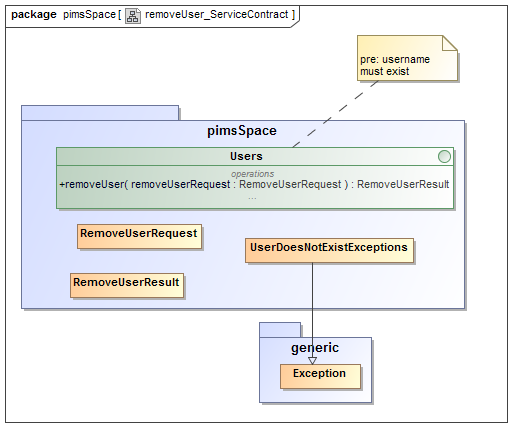
\includegraphics[width=0.7\linewidth]{./Functional_Requirements/Graphics/pimsSpace/removeUser_ServiceContract}}
			\caption{Service contract for removeUser}
		\end{figure}
	\end{description} 
\end{description}